% Capítulo 2: o modelo de maturidade de Richardson, em degraus.
\documentclass[border=4pt]{standalone}
\usepackage[utf8]{inputenc}
\usepackage[T1]{fontenc}
% Estilo comum dos fluxogramas e diagramas de blocos.
\usepackage{tikz}
\usetikzlibrary{arrows.meta, positioning, calc, shapes.geometric, shapes.misc}
\definecolor{navy}{RGB}{23,45,80}
\definecolor{laranja}{RGB}{250,110,29}
\definecolor{cinzalogo}{RGB}{107,114,126}
\definecolor{azul}{RGB}{205,222,247}
\tikzset{
  base/.style={draw=navy, line width=0.9pt, font=\sffamily\small, align=center, inner sep=4pt},
  terminal/.style={base, rounded rectangle, fill=laranja!45, draw=laranja, minimum width=20mm, minimum height=7mm},
  processo/.style={base, rectangle, fill=laranja!12, minimum width=28mm, minimum height=8mm},
  decisao/.style={base, diamond, aspect=2.2, fill=azul, inner sep=1pt, minimum width=30mm},
  es/.style={base, trapezium, trapezium left angle=72, trapezium right angle=108,
             fill=white, minimum width=26mm, minimum height=8mm, trapezium stretches body},
  fluxo/.style={-{Stealth[length=2.2mm]}, navy, line width=0.9pt},
  rotulo/.style={font=\sffamily\small\bfseries, text=navy},
  legenda/.style={font=\sffamily\scriptsize, text=cinzalogo},
  resposta/.style={font=\sffamily\scriptsize\bfseries, text=navy},
}

\tikzset{
  degrau/.style={base, rectangle, anchor=south west, minimum width=26mm, align=left, text width=23mm, font=\sffamily\scriptsize},
  nivel/.style={font=\sffamily\small\bfseries, text=navy},
}
\begin{document}
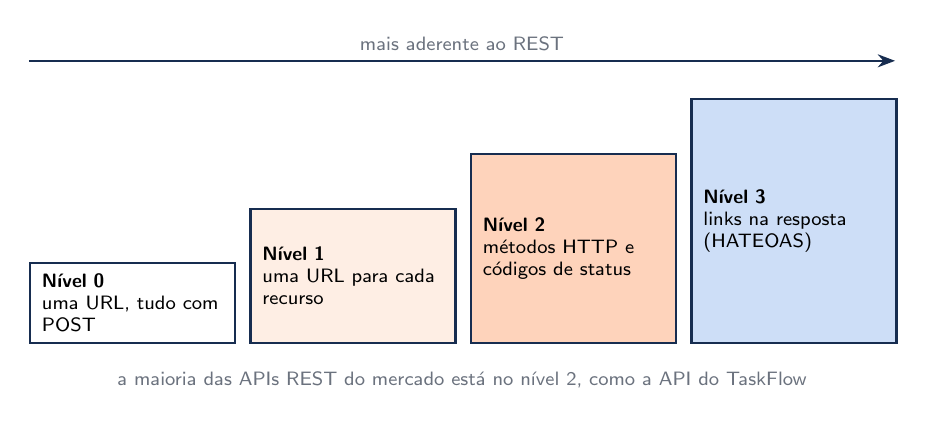
\begin{tikzpicture}
  \node[degrau, fill=white, minimum height=10mm] at (0, 0)
    {\textbf{Nível 0}\\uma URL, tudo com POST};
  \node[degrau, fill=laranja!12, minimum height=17mm] at (2.8, 0)
    {\textbf{Nível 1}\\uma URL para cada recurso};
  \node[degrau, fill=laranja!30, minimum height=24mm] at (5.6, 0)
    {\textbf{Nível 2}\\métodos HTTP e códigos de status};
  \node[degrau, fill=azul, minimum height=31mm] at (8.4, 0)
    {\textbf{Nível 3}\\links na resposta (HATEOAS)};
  \draw[fluxo] (0, 3.6) -- node[above, legenda] {mais aderente ao REST} (11, 3.6);
  \node[legenda] at (5.5, -0.45) {a maioria das APIs REST do mercado está no nível 2, como a API do TaskFlow};
\end{tikzpicture}
\end{document}
